\documentclass[8pt]{beamer}

\usepackage[utf8]{inputenc}
\usepackage[T1]{fontenc}

\usepackage{longtable}
\usepackage{booktabs}

\usepackage{graphicx}
\usepackage{subfig}
\usepackage{floatrow}
\captionsetup{labelsep=period}

\usepackage{standalone}

\usepackage{amssymb, amsmath, mathrsfs, mathtools, dsfont, bbold}

\usetheme{ign}

\title{Classification et apprentissage statistique}
\subtitle{Supervisé et non-supervisé}
\author{Oussama ENNAFII}
\institute{ENSG}
\date{\today}

\begin{document}

	\begin{frame}[plain]
		\titlepage{}
	\end{frame}

	\section{Introduction}

		\begin{frame}{Classer: première définition}
			Champs lexical
			\begin{itemize}
				\item<2-> ranger,
				\item<3-> labeliser,
				\item<4-> catégoriser,
				\item<5-> hiérarchiser.
			\end{itemize}
			\only<6->{
				\begin{block}{Esquisse de définition}
					Classer: ranger $n$ \textbf{objets} dans $k$ \textbf{catégories} (avec $k << n$).
				\end{block}
			}
		\end{frame}
		
		\begin{frame}{Comment classer?}
			\begin{itemize}
					\item<1-> Comment caractériser un objet à classer?
					\item<2-> Comment sont-elle définit les catégories (ou classes) d'objets?
			\end{itemize}
		\end{frame}

		\begin{frame}{Exemples de problèmes de classifications}
			\begin{figure}[H]
				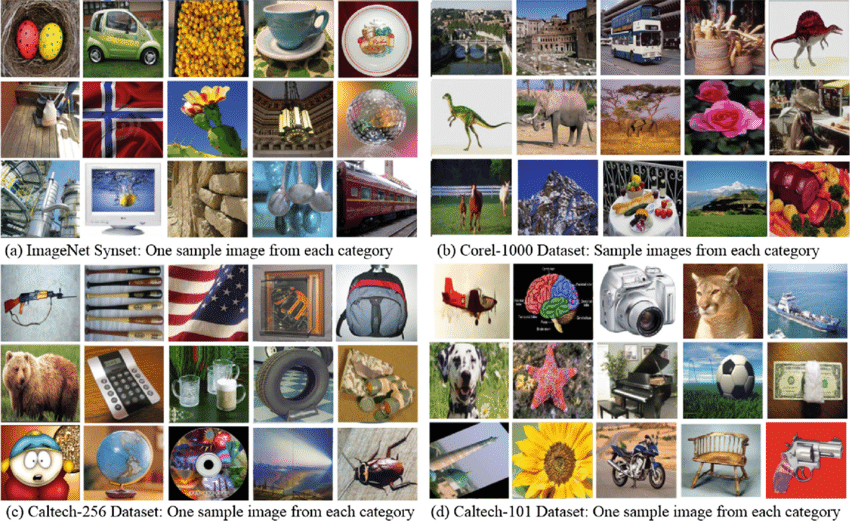
\includegraphics[width=.7\textwidth]{images/samples/image_datasets}
				\caption*{\tiny Exemples de base de données d'images~\cite{ahmed2017fusion}.}
			\end{figure}
		\end{frame}
		
		\begin{frame}{Exemples de problèmes de classifications}
			\begin{figure}[H]
				\ffigbox[\FBwidth]
				{
					\begin{subfloatrow}[2]
						\ffigbox[\FBwidth]
						{
							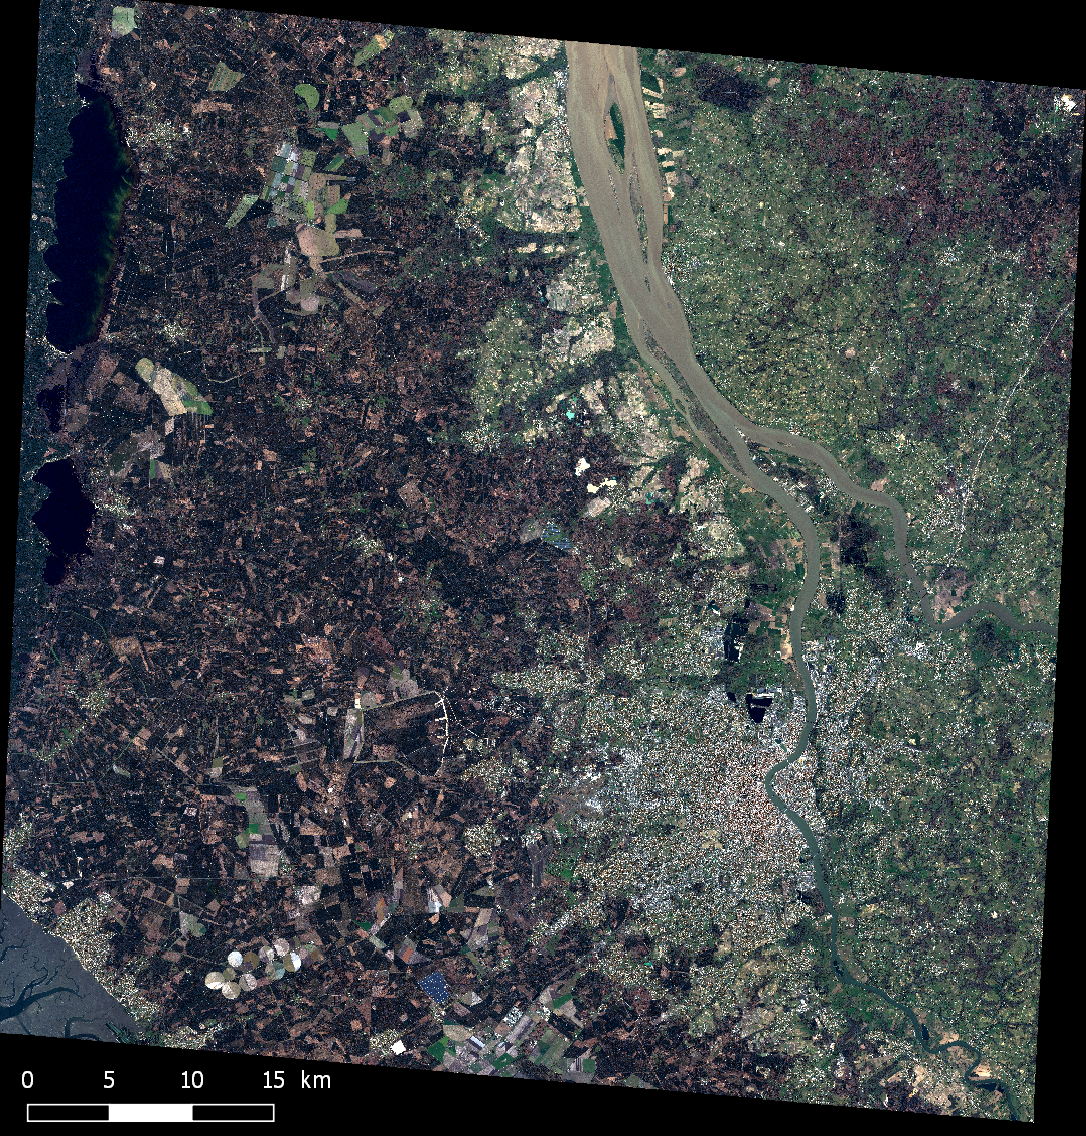
\includegraphics[width=.31\textwidth]{images/samples/gironde}
						}
						{
							\caption*{\tiny Image de la Gironde prise par SPOT en 2016: Résolution $1.5m$, $4$ canaux: \{{\color{purple!20}Infrarouge}, {\color{red}Rouge}, {\color{green}Vert}, {\color{blue}Bleu}\}.}
						}
						\ffigbox[\FBwidth]
						{
							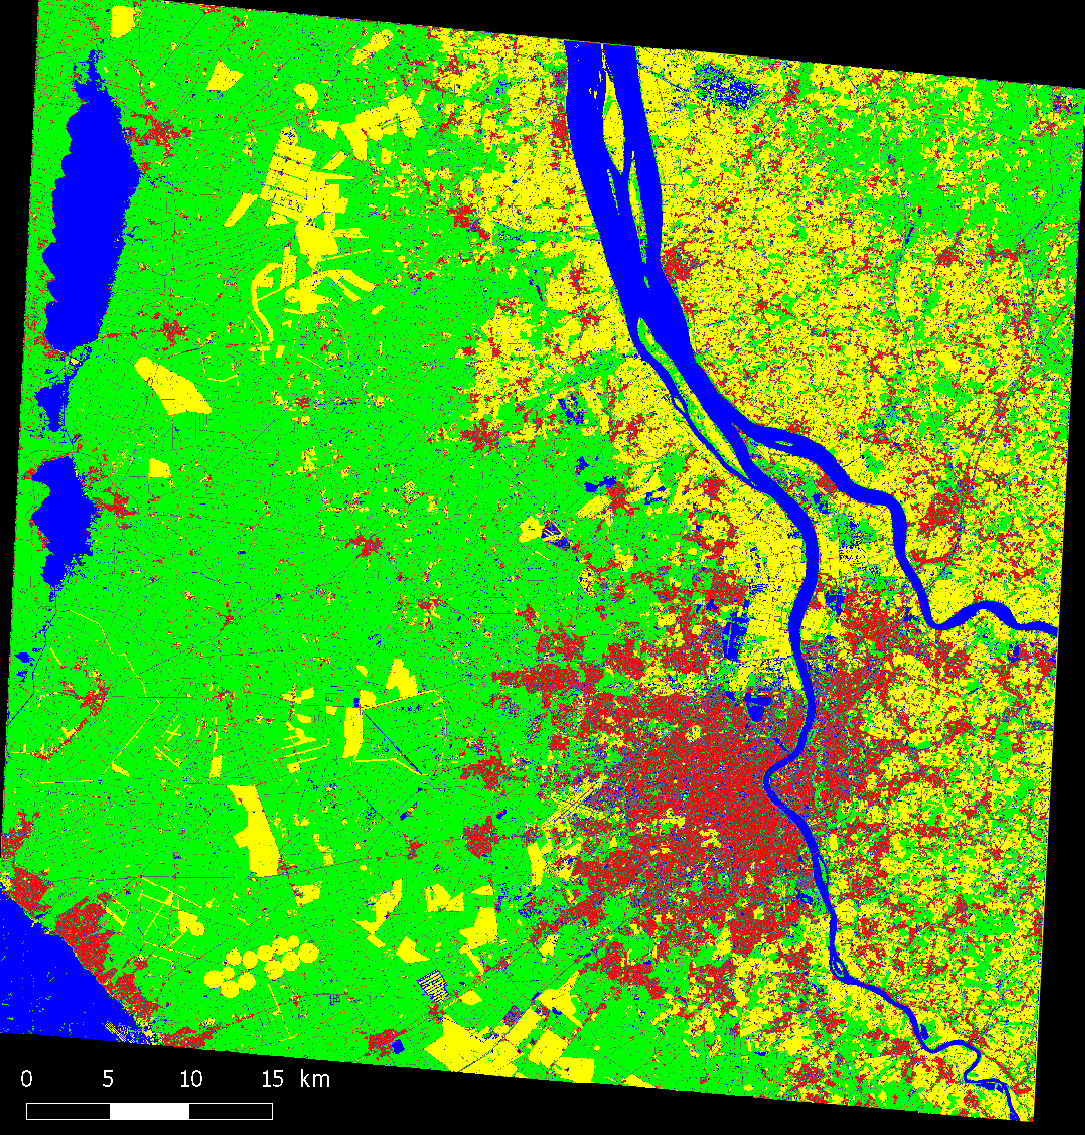
\includegraphics[width=.31\textwidth]{images/samples/gironde_classif}
						}
						{
							\caption*{\tiny Occupation des sols extraite de l'image: {\color{red}$\blacksquare$} Bâti, {\color{green}$\blacksquare$} Forêt, {\color{yellow}$\blacksquare$} Culture, {\color{gray}$\blacksquare$} Routes, {\color{blue}$\blacksquare$} Eau.}
						}
					\end{subfloatrow}
				}
				{
					\caption*{\tiny Classification appliquée pour l'Occupation des sols~\cite{postadjian2017investigating}.}
				}
			\end{figure}
		\end{frame}

		\begin{frame}{Exemples de problèmes de classifications}
			\begin{figure}[H]
				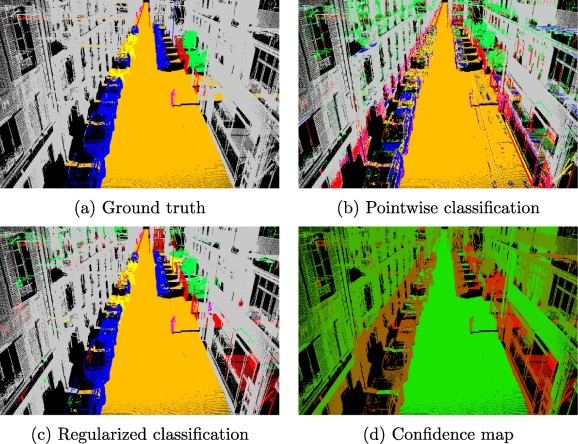
\includegraphics[width=.6\textwidth]{images/samples/pc_classification}
				\caption*{\tiny Exemple de classification de nuage de point\cite{landrieu2017structured}.}
			\end{figure}
		\end{frame}

		\begin{frame}{Exemples de problèmes de classifications}
			\begin{figure}[H]
				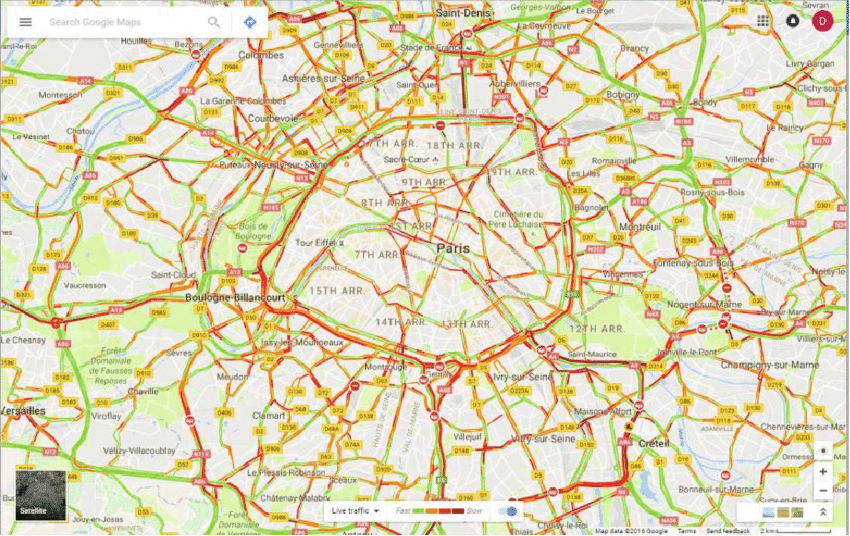
\includegraphics[width=.65\textwidth]{images/samples/traffic_paris}
				\caption*{\tiny Exemple de classification utilisé pour déterminer les conditions de circulation à Paris le 06/09/2016 à 9:30~\cite{tutic2016google}.}
			\end{figure}
		\end{frame}


	% \begin{frame}{Rappel: Classification supervisée}
	% 	\begin{figure}[H]
	% 		\begin{center}
	% 			\includestandalone[mode=buildnew, height=.4\textheight]{scatter_gender_dataset}
	% 			\caption*{\tiny Exemple de problème de classification: $2$ attributs et $2$ classes.}
	% 		\end{center}
	% 	\end{figure}
	% 	\begin{itemize}
	% 		\item <1-> On observe $n$ échantillons: $\big((X^i, Y^i)\big)_{i=1,\dots,n}$
	% 		\item <2-> Connaissant une instance $X^j = \begin{pmatrix}
	% 		X_1^j\\
	% 		\vdots \\
	% 		X_d^j
	% 		\end{pmatrix}$, il faut prédire sa classe $Y^j$ et la probabilité de cette classe.
	% 	\end{itemize}
	% \end{frame}

	% \begin{frame}{Supervisé vs Non-Supervisée}
	% 	\begin{figure}[H]
	% 		\begin{center}
	% 			\includestandalone[mode=buildnew, height=.4\textheight]{scatter_circles}
	% 			\caption*{\tiny Exemple de problème de classification non supervisée: Pas de classes mais une structure se dégage.}
	% 		\end{center}
	% 	\end{figure}
	% 	\begin{itemize}
	% 		\item <1-> On observe ${(X^i)}_{i=1,\dots,n}$ sans les classes $\longrightarrow$ non supervisée,
	% 		\item <2-> On observe ${\big((X^i, Y^i)\big)}_{i=1,\dots,n}$ $\longrightarrow$ supervisée.
	% 	\end{itemize}
	% \end{frame}

	% \begin{frame}{Discriminatif vs Génératif}
	% 	On suppose que ${\big((X^i, Y^i)\big)}_{i=1,\dots,n}$ sont des réalisations indépendantes et identiquement distribuées (i.i.d) de la loi $\mathbb{P}(X=x, Y=y) = p(x,y)$.
	% 	\begin{itemize}
	% 		\only<1-5>{
	% 			\item <1-> On sait modéliser la distribution des classes $p(y)$ et celle des instances selon la classe $p(x\vert y)$ $\longrightarrow$ méthode générative,
	% 			\begin{itemize}
	% 				\item <2-> Exemple: On s'interresse à la detection de sexe selon deux mesures: taille et poids.
	% 				\item <3-> On suppose que la répartition des sexes est équilibrée dans le monde $p(y=1) = p(y=0) = \frac{1}{2}$ et que et que la répartition des mesures suivent des lois gaussiennes $X\vert Y \sim \mathscr{N}(m_y, \sigma_y)$;
	% 				\item <4-> On infère la probabilité $p(y \vert x) = \frac{p(x\vert y). p(y)}{p(x)}$.
	% 				\item <5-> On choisit la plus probable: $\arg \max_{y} p(y \vert x)$.
	% 			\end{itemize}
	% 		}
	% 		\only<6-7>{
	% 			\item <6-> On n'a aucune connaissance \textit{a priori}. On cherche à apprendre un modèle de $p(y \vert x)$ $\longrightarrow$ méthode discriminative,
	% 			\begin{itemize}
	% 				\item <7-> Exemple: On apprend un modèle d'arbres aléatoires.
	% 			\end{itemize}
	% 		}
	% 	\end{itemize}
	% \end{frame}

	% \begin{frame}{Pourquoi classifier?}
	% 	
	% \end{frame}


	% \section[SVM]{SVM}
	% \begin{frame}{Curse of dimensionality}
	% 	\begin{itemize}
	% 		\item <1-> Si on a $n$ points à séparer, sans aucun modèle de classification, il y a un nombre exponentiel de séparations $ \frac{\vert \mathscr{P}(\{1,\dots,n\}) \vert}{2} = 2^{n-1}$ possibles $\longrightarrow$ C'est incalculable.
	% 		\item <2-> Il faut donc un modèle de séparation qui permettra de chercher efficacement une bonne solution: Forêts Aléatoires, \textbf{SVM}, Réseaux de Neurones \dots
	% 	\end{itemize}
	% \end{frame}
	% \subsection{Un peu de théorie}
	% 	\begin{frame}{Régresser sur les probabilité: fausse bonne idée.}
	% 		\begin{itemize}
	% 			\item<1-> On impose un modèle de probabilité $p(y\vert x)$.
	% 				\begin{itemize}
	% 					\item régression de densité parametrique: Bernoulli, Poisson \dots;
	% 					\item régression de densité non-parametrique.
	% 				\end{itemize}
	% 			\item<2-> \textcolor{red}{Problème: on impose trop d'hypothèses contraignantes.}
	% 			\item<3-> Comment faire? Quels types d'hypothèse à choisir?
	% 		\end{itemize}
	% 	\end{frame}
	% 	\begin{frame}{Formalisation: fonction de décision}
	% 		\begin{itemize}
	% 			\item<1-> On se place dans le cas de classification binaire:
	% 				$$ X^i \in \mathbb{R}^d , \quad \forall i=1,\dots,n$$
	% 				$$ Y^i \in \{-1, +1\} , \quad \forall i=1,\dots,n$$
	% 				$$\eta(x) = p(y = 1 \vert x) = 1 - p(y = -1 \vert x), \quad \forall x \in \mathbb{R}^d$$
	% 			\item<2-> On cherche une fonction de décision $D$ comme suit:
	% 			\begin{align*}
	% 				D: \mathbb{R}^d &\rightarrow \{-1, +1\} \\
	% 				x &\mapsto D(x)
	% 			\end{align*}
	% 			\item<3-> On définit le regret, ou risque, d'une fonction de décision $D$ par:
	% 			\begin{equation}
	% 				R(D) \triangleq \mathbb{E}_{X,Y}(\mathbb{1}(D(X)\neq Y))
	% 			\end{equation}
	% 			\item<4-> Cette fonction calcule la mesure de l'espace d'attributs où $D(x) \neq y$:
	% 			\begin{align*}
	% 				R(D) &= \mathbb{P}(\{D(X)\neq Y\})\\
	% 					 &= \sum_{y\in \{-1, 1\}} \int_{x \in \mathbb{R}^d} \mathbb{1}(D(x)\neq y) p(dx, y)
	% 			\end{align*}
	% 		\end{itemize}
	% 	\end{frame}
	% 	\begin{frame}{Fonction de décision optimal}
	% 		\begin{itemize}
	% 			\item<1-> Le "décideur" optimal $D^*$ donne le regret $R(D^*)$ minimal:
	% 				  \begin{equation}
	% 					  D^* \triangleq \arg \min_{D} R(D) 
	% 				  \end{equation}
	% 			\item<2-> On appelle cette fonction la fonction de décision de Bayes. On prouve que:
	% 				  \begin{equation}
	% 					D^*(x) \triangleq 2.\mathbb{1}(\eta(x) > \frac{1}{2}) - 1
	% 				  \end{equation}
	% 			\item<3-> En pratique, on ne connait pas $\eta: \mathbb{R}^d \rightarrow [0,1]$.
	% 		\end{itemize}
	% 	\end{frame}

	% 	\begin{frame}{Apprentissage de séparateur}
	% 		\begin{itemize}
	% 			\item<1-> On évite de modéliser $\eta$ sur tout l'espace d'attributs $\mathbb{R}^d$.
	% 			\item<2-> Il est plus judicieux de modèliser $\eta$ sur les points $x$ où:
	% 					\begin{equation*}
	% 						\eta(x) = \frac{1}{2}
	% 					\end{equation*}
	% 			\item<3->  Cela revient à étudier ce qu'on appelle un séparateur; i.e. la courbe qui vérifie:
	% 				\begin{equation}
	% 					\mathscr{S}_{binary} \triangleq \{X \in \mathbb{R}^d: \eta(x) = \frac{1}{2} \}
	% 				\end{equation}
	% 		\end{itemize}
	% 	\end{frame}

	% 	\begin{frame}{Séparateur: illustration}
	% 		\begin{figure}[H]
	% 			\includestandalone[mode=buildnew, width=.5\textwidth]{scatter_separators}
	% 			\caption*{\tiny Séparateurs possibles des données. $\mathscr{S}_1$ est un exemple de séparateur courbe alors que $\mathscr{S}_2$ est un séparateur linéaire.}
	% 		\end{figure}
	% 	\end{frame}

	% 	\begin{frame}{Choix du séparateur}
	% 		\begin{itemize}
	% 			\item  Il y a une infinité de modèle de $D$ possible.
	% 			\item  Un choix naïf serait de donner, pour chaque instance d'entraînement $X^i$, la valeur qui lui est associé $Y^i$, et pour toute autre valeur $x$ une classe de façon aléatoire:
	% 			\begin{equation*}
	% 				D_n(x) = \sum_{i=1,\dots,n} Y^i . \delta_{X^i}(x) + b . \mathbb{1}_{x \notin \{X^i, \forall i=1,\dots,n\}}
	% 			\end{equation*}
	% 			où: $b \sim \mathscr{B}(0.5)$ est une valeur aléatoire qui suit une loi de Bernoulli avec paramètre $0.5$.
	% 			\item Cependant, ce classifieur n'a aucun pourvoir de généralisation. En effet:
	% 			\begin{gather*}
	% 				\widetilde{x} := \sum_{i=1,\dots,n} X^i \notin \{X^i, \forall i=1,\dots,n\} \\
	% 				\Rightarrow D_n(\widetilde{x}) \sim \mathscr{B}(0.5)
	% 			\end{gather*}
	% 			\item  On réduit, dans le cadre du cours, le choix des séparateurs à ceux qui sont linéaires:
	% 			\begin{align*}
	% 				D_{\textbf{w}, b}: \mathbb{R}^d &\rightarrow \{-1, +1\} \\
	% 				\textbf{x} &\mapsto D_{\textbf{w}, b}(\textbf{x}) = 2.\mathbb{1}(\textbf{w}.\textbf{x} + b > 0) - 1
	% 			\end{align*}
	% 		\end{itemize}
	% 	\end{frame}

	% \subsection[linear]{SVM linéaire}
	% 	\begin{frame}{Mais c'est quoi donc ce SVM?}
	% 		\begin{itemize}
	% 			\item  SVM\@: Support Vector Machines.
	% 			\item  C'est quoi donc un vecteur support?
	% 			\item  Quelle est la relation avec les séparateurs linéaires?
	% 		\end{itemize}
	% 	\end{frame}

	% 	\begin{frame}{SVM\@: maximiser la marge.}
	% 		\begin{figure}[H]
	% 			\includegraphics[width=\textwidth]{images/samples/svm}
	% 			\caption*{ Le séparateur linéaire SVM.}
	% 		\end{figure}
	% 	\end{frame}

	% 	\begin{frame}{SVM\@: maximiser la marge.}
	% 		\begin{itemize}
	% 			\item  Le but du SVM est de maximiser la marge~\cite{vapnik1998statistical}.
	% 			\item  On remarque que:
	% 			\begin{gather*}
	% 				(\textbf{w}, b) \in \{\omega \in \mathbb{R}^d : \omega.\textbf{x} + b = 0\} \\
	% 				\Rightarrow
	% 				(\lambda . \textbf{w}, \lambda.b) \in \{\omega \in \mathbb{R}^d : \omega.\textbf{x} + b = 0\}\quad, \forall \lambda \in \mathbb{R}\setminus\{0\}
	% 			\end{gather*}
	% 			\item  Il y a donc une infinité de solutions possibles. On prend donc la solution $\textbf{w}$ qui permet d'avoir:
	% 			\begin{align}
	% 				\textbf{w}.\textbf{x}_{\color{blue}+} + b &= {\color{blue}+}1 \\
	% 				\textbf{w}.\textbf{x}_{\color{red}-} + b &= {\color{red}-}1
	% 			\end{align}
	% 			où:
	% 			\begin{itemize}
	% 				\item[{\color{blue}+}] $\textbf{x}_{\color{blue}+}$ correspond aux vecteurs supports positifs (i.e. $Y={\color{blue}+}1$).
	% 				\item[{\color{red}---}] $\textbf{x}_{\color{red}-}$ correspond aux vecteurs supports négatifs (i.e. $Y={\color{red}-}1$).
	% 			\end{itemize}
	% 		\end{itemize}
	% 	\end{frame}

	% 	\begin{frame}[plain]{SVM\@: maximiser la marge}
	% 		\begin{figure}[H]
	% 			\includestandalone[mode=buildnew, width=.75\textwidth]{svm_separable}
	% 			\caption*{\tiny Le séparateur linéaire SVM.}
	% 		\end{figure}
	% 	\end{frame}

	% 	\begin{frame}{La marge}
	% 		\begin{itemize}
	% 			\only<1>{
	% 				\item  La marge est la longueur de la projection orthogonal de $(\textbf{x}_+ - \textbf{x}_-)$ sur la droite porter par $\textbf{w}$:
	% 					\begin{align*}
	% 					M &= \frac{\textbf{w}}{\vert\vert \textbf{w} \vert\vert}.(\textbf{x}_+ - \textbf{x}_-) \\
	% 					&= \frac{\textbf{w}.\textbf{x}_+ - \textbf{w}.\textbf{x}_-}{\vert\vert \textbf{w} \vert\vert}\\
	% 					&= \frac{\textbf{w}.\textbf{x}_+ + b - (\textbf{w}.\textbf{x}_- + b)}{\vert\vert \textbf{w} \vert\vert}\\
	% 					&= \frac{2}{\vert\vert \textbf{w} \vert\vert}
	% 					\end{align*}
	% 			}
	% 			\item<2-> La marge est la longueur de la projection orthogonal de $(\textbf{x}_+ - \textbf{x}_-)$ sur la droite porter par $\textbf{w}$:
	% 				\begin{equation}
	% 					M = \frac{2}{\vert\vert \textbf{w} \vert\vert}
	% 				\end{equation}
	% 			\item<2->  Le problème posé par le SVM est donc formulé comme suit:
	% 			\begin{equation}
	% 				\begin{aligned}
	% 				& \max_{\textbf{w}}
	% 				& & \frac{2}{\vert\vert \textbf{w} \vert\vert} \\
	% 				& \text{sous contrainte}
	% 				& & \begin{cases}
	% 					\textbf{w}.\textbf{X}^i + b \leq -1 & Y^i = -1 \\
	% 					\textbf{w}.\textbf{X}^i + b \geq 1 & Y^i = 1
	% 				\end{cases} \; \forall i = 1, \dots, n.
	% 				\end{aligned}
	% 			\end{equation}
	% 			\item<2->  Ou encore:
	% 			\begin{equation}
	% 				\begin{aligned}
	% 				& \min_{\textbf{w}}
	% 				& & {\vert\vert \textbf{w} \vert\vert}^2 \\
	% 				& \text{sous contrainte}
	% 				& & Y^i.(\textbf{w}.\textbf{X}^i + b) \geq 1 \; \forall i = 1, \dots, n.
	% 				\end{aligned}
	% 			\end{equation}
	% 		\end{itemize}
	% 	\end{frame}

	% 	\begin{frame}{Cas non séparable.}
	% 		\begin{figure}[H]
	% 			\includegraphics[width=\textwidth]{images/samples/non_separable}
	% 			\caption*{\label{fig::non_sep} Le séparateur linéaire SVM.}
	% 		\end{figure}
	% 	\end{frame}

	% 	\begin{frame}{Cas non séparable.}
	% 		\begin{figure}[H]
	% 			\includegraphics[width=\textwidth]{images/samples/stable_margin}
	% 			\caption*{\label{fig::stable_margin} La marge du séparateur linéaire SVM.}
	% 		\end{figure}
	% 	\end{frame}

	\section{Références}
	\begin{frame}[allowframebreaks]{Références}
		\nocite{sklearn_api}
		\bibliographystyle{apalike}
		\bibliography{references.bib}
	\end{frame}

\end{document}
